\section{Summary}
\label{se:method_summary}

\begin{figure}[htp]
    \centering
    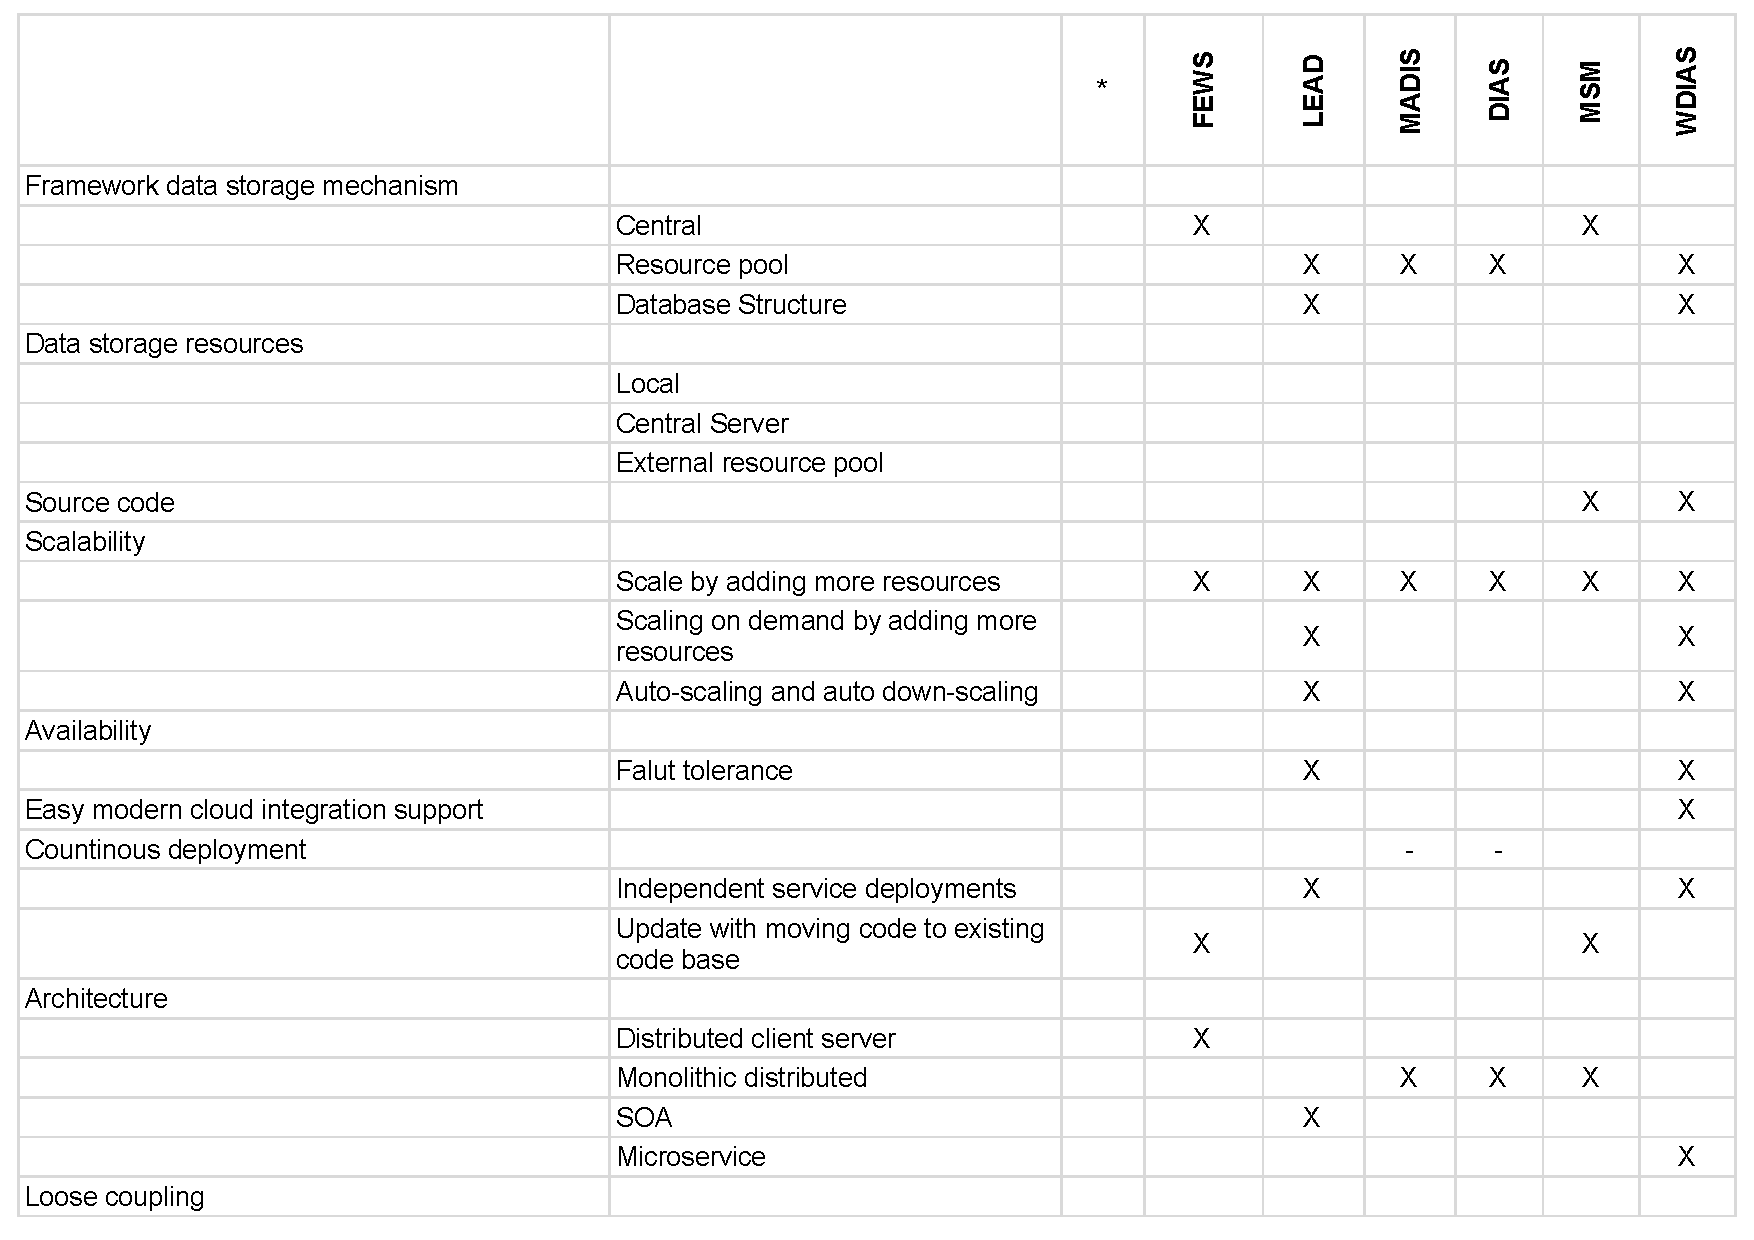
\includegraphics[width=1\textwidth]{method/misc/architecture_comparison_pros_cons.pdf}
    \caption{Architectural comparison}
    \label{fi:architecture_comparison_pros_cons}
\end{figure}

Throughout the \cref{ch:method}, we discussed the methodology of designing and implementing the \acrshort{wdias} based on the concepts studied in the literature review of \cref{ch:literature}. We used microservice architecture over \acrshort{soa} with an \acrshort{esb} to avoid the drawback of streaming bulk data through an \acrshort{esb}. To take the full advantage of using the microservices architecture, we moved to container orchestration based architecture rather than building tightly coupled microservices with the actor model. 
While implementing the import and export modules, those modules followed the microservice architecture style of \emph{smart endpoints and dumb pipes}. Each microservice is implemented as a containerized application that can deploy independent of other microservices. Also, we used the microservice architecture pattern of \emph{database per service} by combining different types of database systems to create the \acrshort{wdias} database structure. Further, we provided a comprehensive extension module system that allows users to preprocess data by creating new triggers without any downtime for system configuration. We used a geo indexing mechanism to support geo-search queries and indexed the timeseries metadata to support the search for any timeseries in \acrshort{wdias}.
